% GD32 Edge AI System Architecture — TikZ for LaTeX
\documentclass[tikz,border=5pt]{standalone}
\usepackage{tikz}
\usetikzlibrary{shapes.geometric, arrows, positioning, fit, backgrounds, calc}
\usepackage{xcolor}

\begin{document}
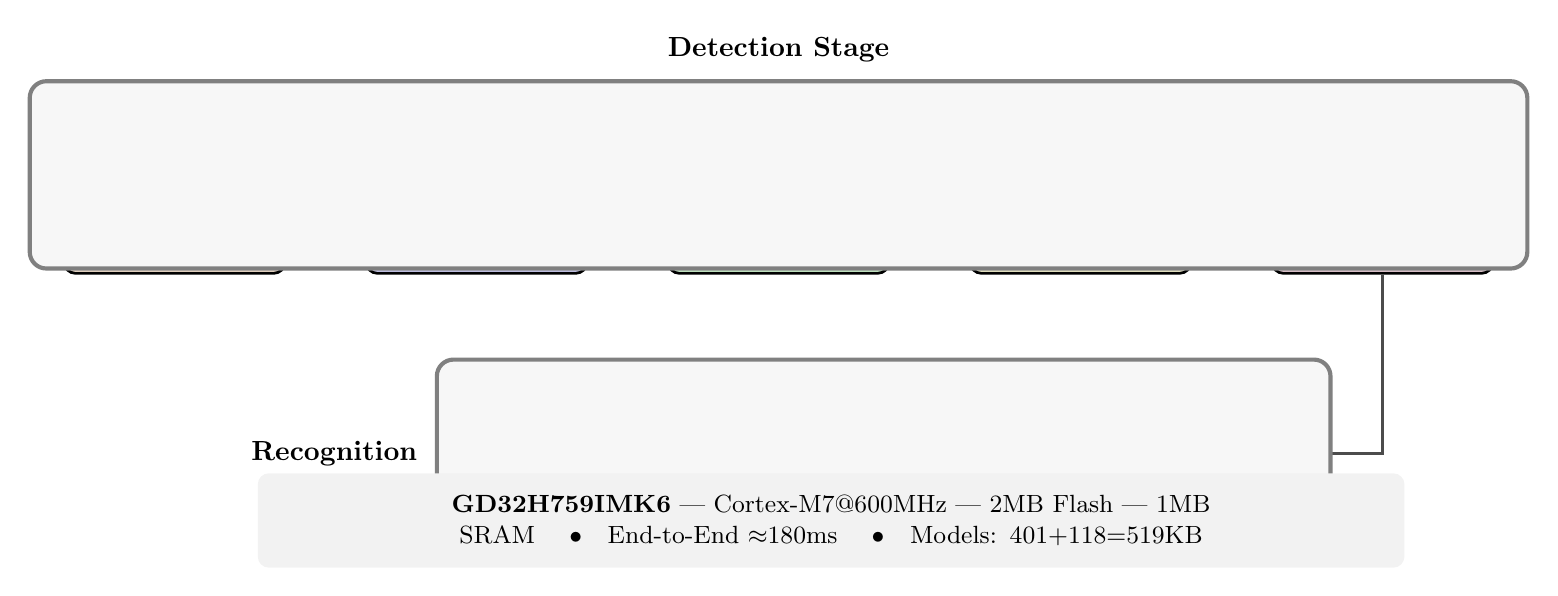
\begin{tikzpicture}[
    block/.style={rectangle, rounded corners=4pt, draw=black, line width=1pt,
                  minimum width=2.8cm, minimum height=1.5cm, align=center, font=\small},
    arrow/.style={->, >=stealth, line width=1.2pt, black!70},
    label/.style={font=\footnotesize\itshape, gray}
]

% === Row 1: Detection Pipeline ===
\node[block, fill=orange!15] (cam) {OV2640 Camera\\800$\times$600 RGB565};
\node[block, fill=blue!15, right=1.0cm of cam] (dma) {DMA2D Scaler\\192$\times$192\\uint8$\to$int8};
\node[block, fill=green!15, right=1.0cm of dma] (yolo) {YOLO-FastestV2\\INT8 401KB\\$\sim$131ms};
\node[block, fill=yellow!15, right=1.0cm of yolo] (dec) {Decode + NMS\\3 anchors/scale\\K-means};
\node[block, fill=purple!15, right=1.0cm of dec] (crop) {Crop Plate\\Gray + 94$\times$24\\uint8$\to$int8};

\draw[arrow] (cam) -- (dma);
\draw[arrow] (dma) -- (yolo);
\draw[arrow] (yolo) -- (dec);
\draw[arrow] (dec) -- (crop);

% Data labels
\node[label, above=0.15cm of $(dma.north)!0.5!(yolo.north)$] {192$\times$192 RGB int8};
\node[label, above=0.15cm of $(dec.north)!0.5!(crop.north)$] {crop coords};

% === Row 2: Recognition Pipeline ===
\node[block, fill=green!15, below=1.5cm of crop, xshift=-2.5cm] (lpr) {LPRNet Tiny\\INT8 118KB\\$<$50ms};
\node[block, fill=yellow!15, left=1.0cm of lpr] (argmax) {Argmax Decode\\VOCAB lookup\\7-char output};
\node[block, fill=pink!15, left=1.0cm of argmax] (disp) {LCD Display\\+ UART};

\draw[arrow] (crop.south) |- (lpr.east);
\draw[arrow] (lpr) -- (argmax);
\draw[arrow] (argmax) -- (disp);

% === Hardware Box ===
\node[draw=black!50, line width=1.5pt, rounded corners=6pt,
      fill=black!3, inner sep=12pt,
      fit=(cam)(dma)(yolo)(dec)(crop), yshift=0.5cm] (det) {};
\node[above=0.1cm of det.north, font=\bfseries] {Detection Stage};

\node[draw=black!50, line width=1.5pt, rounded corners=6pt,
      fill=black!3, inner sep=12pt,
      fit=(lpr)(argmax)(disp)] (rec) {};
\node[left=0.1cm of rec.west, font=\bfseries, anchor=east] {Recognition};

% === Hardware Info ===
\node[below=0.8cm of $(det.south)!0.5!(rec.south)$, font=\small,
      fill=gray!10, rounded corners=4pt, inner sep=8pt,
      text width=14cm, align=center] {
    \textbf{GD32H759IMK6} | Cortex-M7@600MHz | 2MB Flash | 1MB SRAM
    \quad$\bullet$\quad End-to-End $\approx$180ms \quad$\bullet$\quad Models: 401+118=519KB
};

\end{tikzpicture}
\end{document}
